% Editable native annotations around unchanged verified IDE photographs.
\par
\begin{figure}[htbp]
\centering
\newsavebox{\MARSppmpixelsregistersBox}
\sbox{\MARSppmpixelsregistersBox}{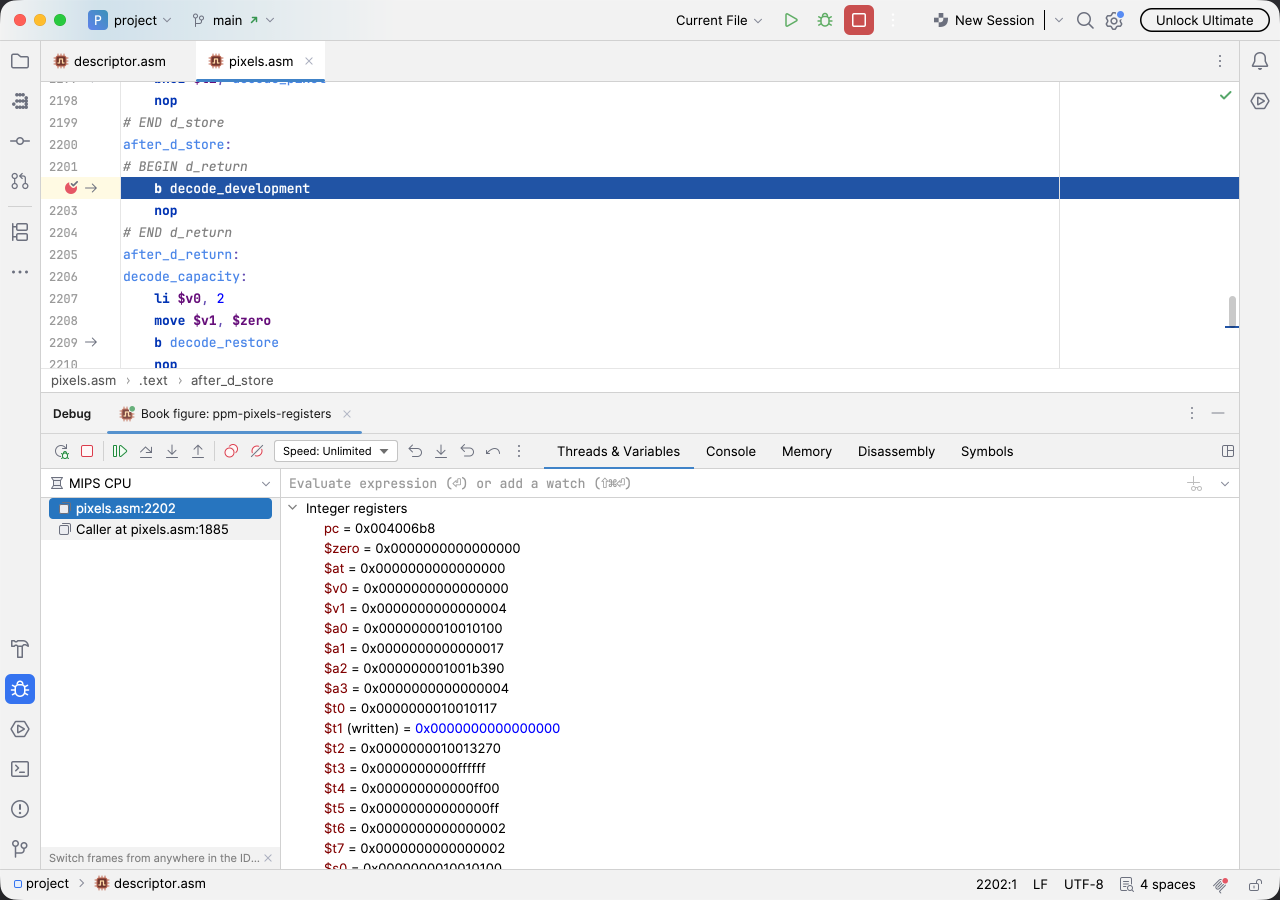
\includegraphics[artifact]{packages/029-binary-ppm/captures/f02/registers.png}}
\newsavebox{\MARSppmpixelssourceBox}
\sbox{\MARSppmpixelssourceBox}{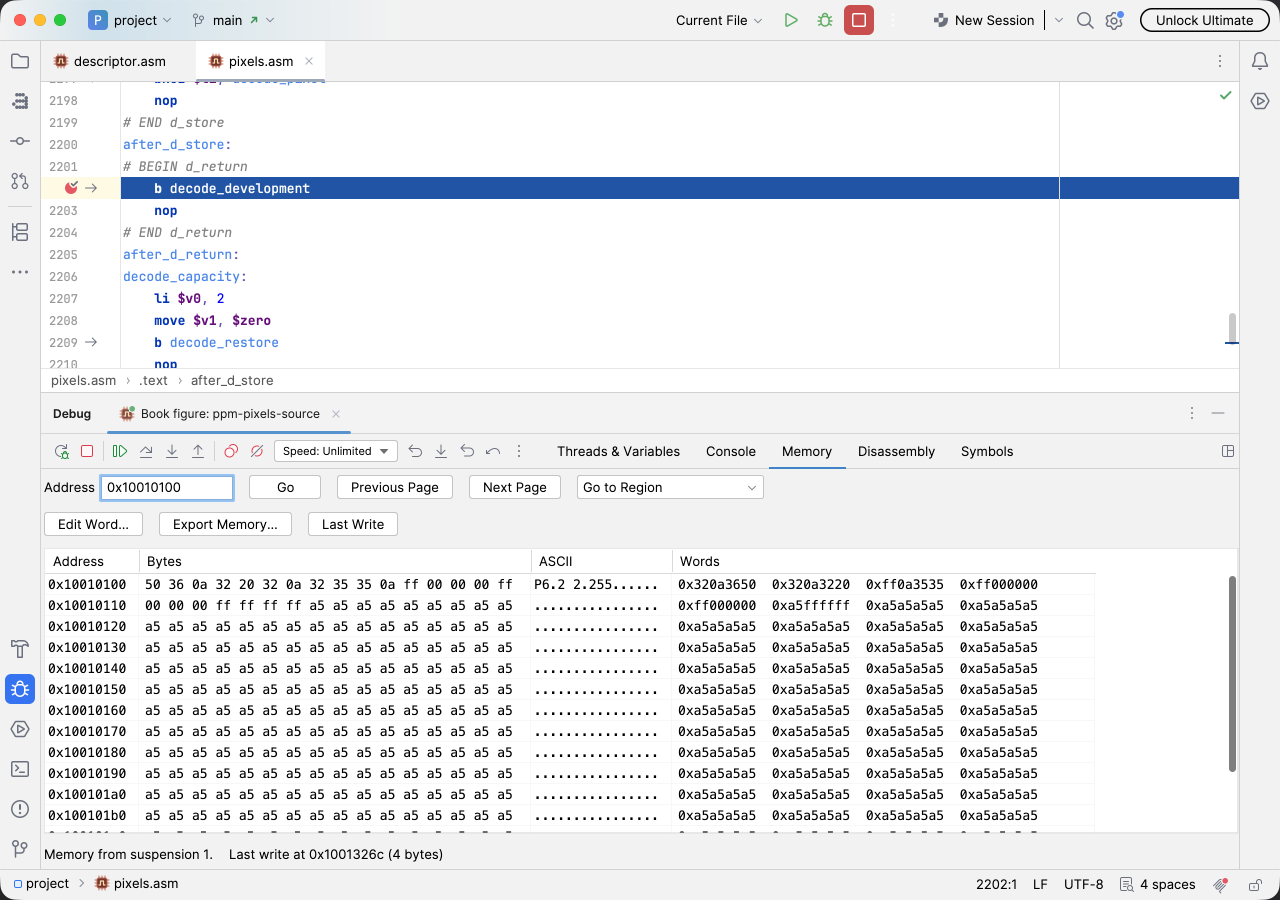
\includegraphics[artifact]{packages/029-binary-ppm/captures/f02/source.png}}
\newsavebox{\MARSppmpixelsframebufferBox}
\sbox{\MARSppmpixelsframebufferBox}{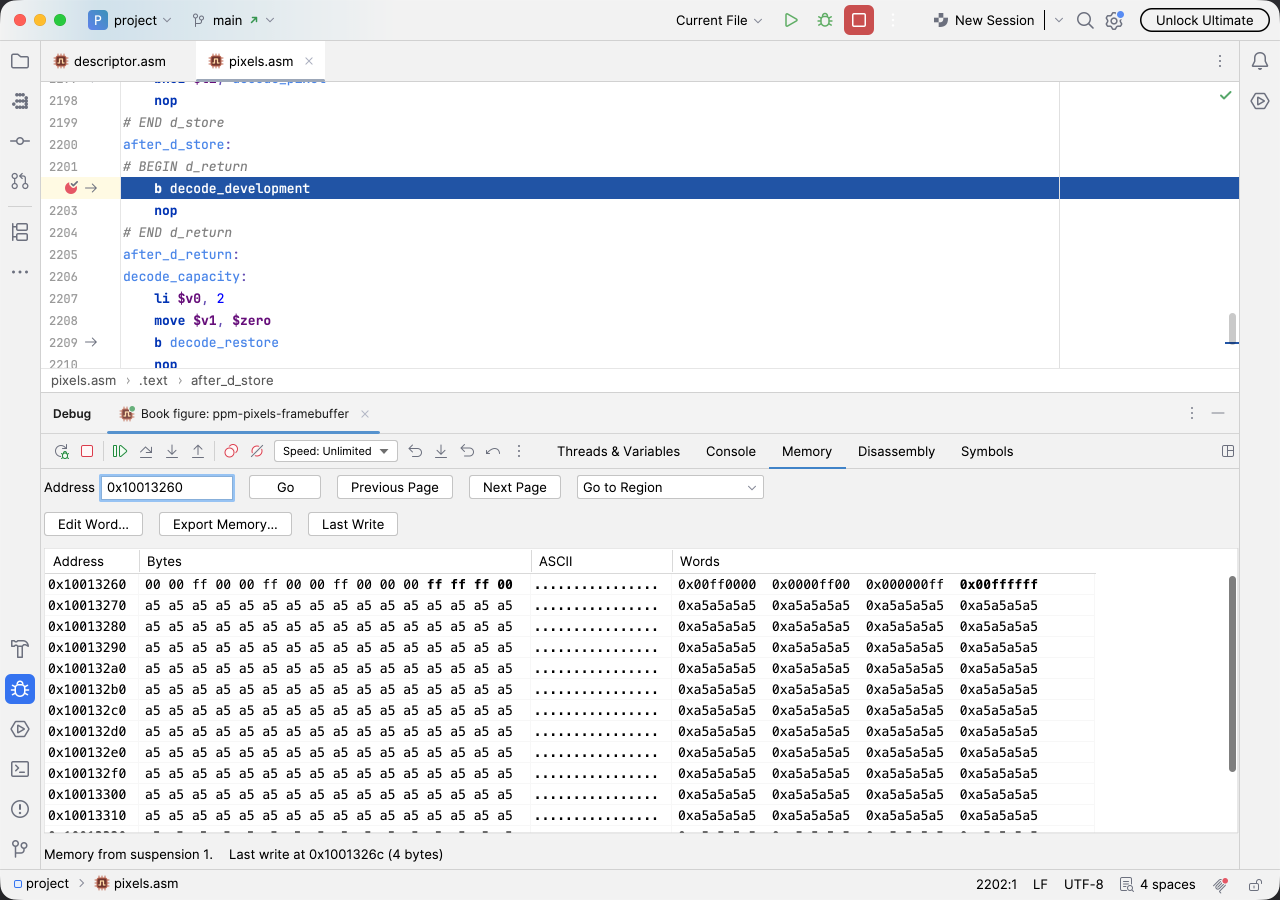
\includegraphics[artifact]{packages/029-binary-ppm/captures/f02/framebuffer.png}}
\newsavebox{\MARSppmpixelsprivateBox}
\sbox{\MARSppmpixelsprivateBox}{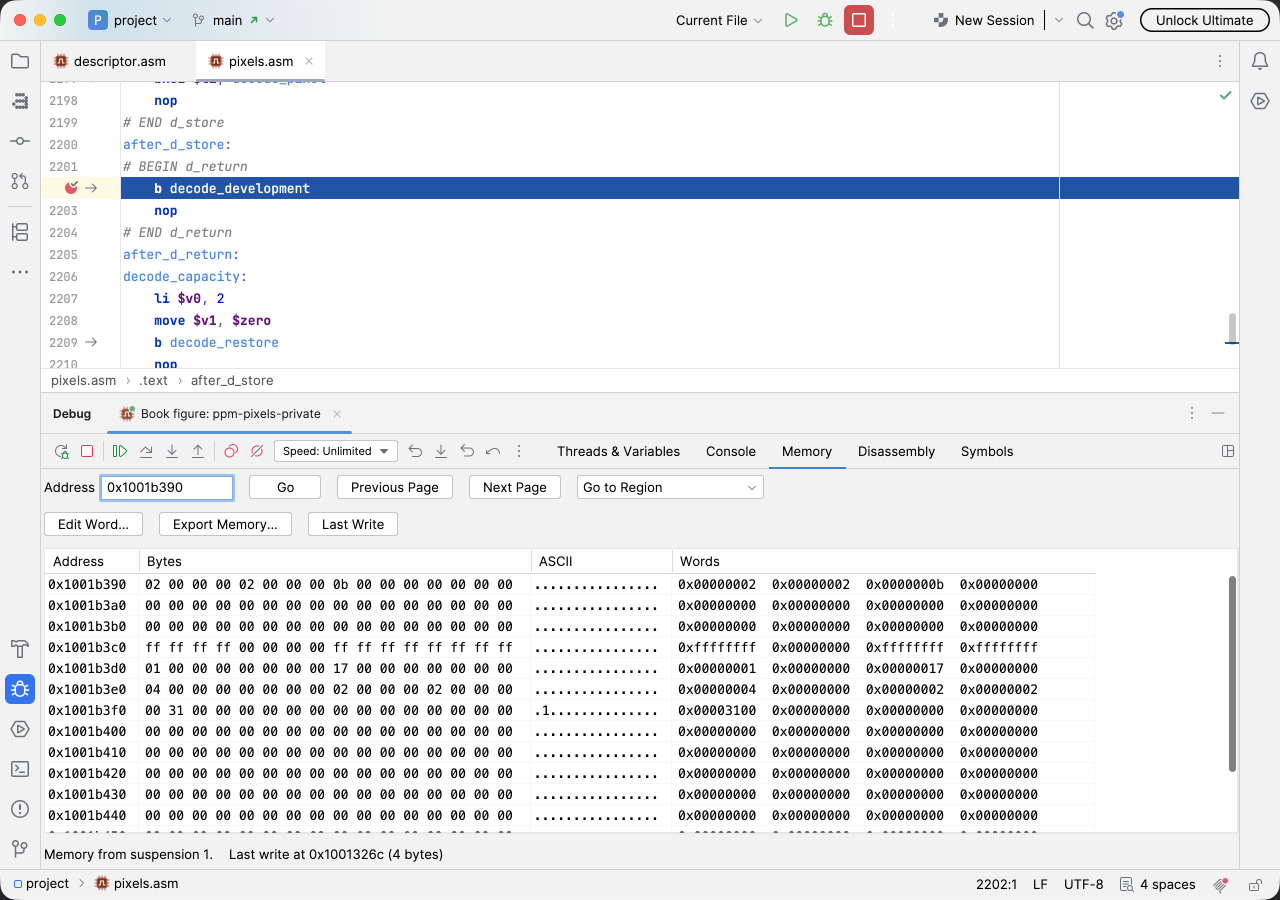
\includegraphics[artifact]{packages/029-binary-ppm/captures/f02/private.png}}
\edef\MARSppmpixelssourceLeft{\the\dimexpr0.036718750\wd\MARSppmpixelsregistersBox\relax}
\edef\MARSppmpixelssourceBottom{\the\dimexpr0.774444444\ht\MARSppmpixelsregistersBox\relax}
\edef\MARSppmpixelssourceRight{\the\dimexpr0.713281250\wd\MARSppmpixelsregistersBox\relax}
\edef\MARSppmpixelssourceTop{\the\dimexpr0.170000000\ht\MARSppmpixelsregistersBox\relax}
\edef\MARSppmpixelscursorsLeft{\the\dimexpr0.246093750\wd\MARSppmpixelsregistersBox\relax}
\edef\MARSppmpixelscursorsBottom{\the\dimexpr0.156666667\ht\MARSppmpixelsregistersBox\relax}
\edef\MARSppmpixelscursorsRight{\the\dimexpr0.553906250\wd\MARSppmpixelsregistersBox\relax}
\edef\MARSppmpixelscursorsTop{\the\dimexpr0.773333333\ht\MARSppmpixelsregistersBox\relax}
\edef\MARSppmpixelsinputLeft{\the\dimexpr0.034375000\wd\MARSppmpixelssourceBox\relax}
\edef\MARSppmpixelsinputBottom{\the\dimexpr0.311111111\ht\MARSppmpixelssourceBox\relax}
\edef\MARSppmpixelsinputRight{\the\dimexpr0.584375000\wd\MARSppmpixelssourceBox\relax}
\edef\MARSppmpixelsinputTop{\the\dimexpr0.608888889\ht\MARSppmpixelssourceBox\relax}
\edef\MARSppmpixelsoutputLeft{\the\dimexpr0.034375000\wd\MARSppmpixelsframebufferBox\relax}
\edef\MARSppmpixelsoutputBottom{\the\dimexpr0.311111111\ht\MARSppmpixelsframebufferBox\relax}
\edef\MARSppmpixelsoutputRight{\the\dimexpr0.584375000\wd\MARSppmpixelsframebufferBox\relax}
\edef\MARSppmpixelsoutputTop{\the\dimexpr0.608888889\ht\MARSppmpixelsframebufferBox\relax}
\edef\MARSppmpixelsmetadataLeft{\the\dimexpr0.034375000\wd\MARSppmpixelsprivateBox\relax}
\edef\MARSppmpixelsmetadataBottom{\the\dimexpr0.334444444\ht\MARSppmpixelsprivateBox\relax}
\edef\MARSppmpixelsmetadataRight{\the\dimexpr0.584375000\wd\MARSppmpixelsprivateBox\relax}
\edef\MARSppmpixelsmetadataTop{\the\dimexpr0.608888889\ht\MARSppmpixelsprivateBox\relax}
\begin{tikzpicture}[alt={Five details after_d_store show the source cursor at the twenty-three-byte end, zero remaining pixels, the framebuffer cursor sixteen bytes past its base, four little-endian color words and private metadata. The unfinished return still produces development status four.}]
\node[anchor=north west,inner sep=0,font=\small\bfseries] (source-title) at (6mm,0) {Next unfinished return region};
\node[anchor=north west,inner sep=0] (source) at ([yshift=-1mm]source-title.south west) {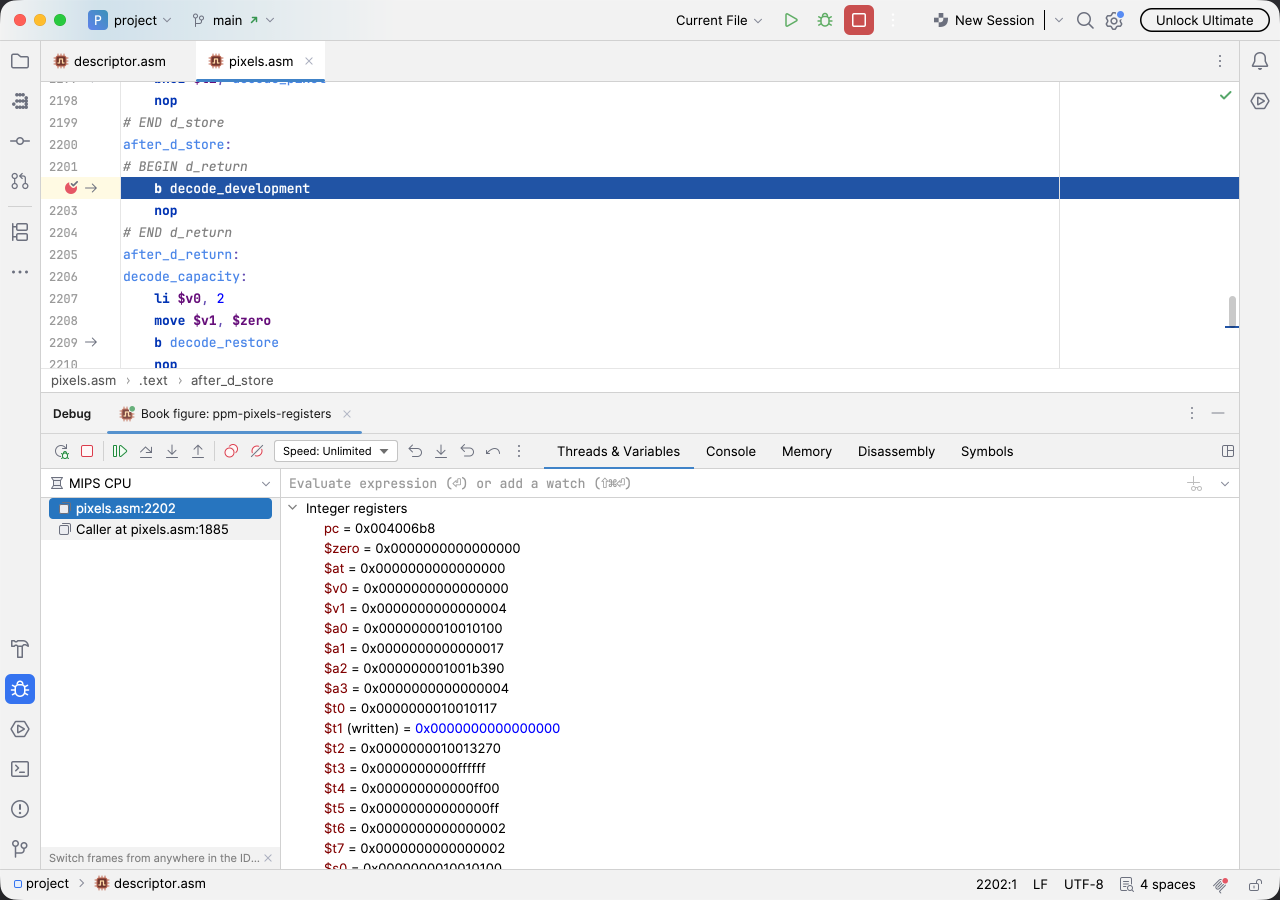
\includegraphics[width=0.54\linewidth,artifact,trim={\MARSppmpixelssourceLeft{} \MARSppmpixelssourceBottom{} \MARSppmpixelssourceRight{} \MARSppmpixelssourceTop{}},clip]{packages/029-binary-ppm/captures/f02/registers.png}};
\begin{scope}[shift={(source.south west)},x={($(source.south east)-(source.south west)$)},y={($(source.north west)-(source.south west)$)}]
\draw[black,line width=0.7pt] (0.237500000,0.080000000) rectangle (0.821875000,0.520000000);
\node[draw=black,fill=white,circle,inner sep=1.5pt,font=\footnotesize] at ($(0.237500000,0.520000000)+(-3mm,0)$) {1};
\end{scope}
\node[anchor=north west,inner sep=0,font=\small\bfseries] (cursors-title) at ([yshift=-1mm]source.south west) {Input end, remaining count and output end};
\node[anchor=north west,inner sep=0] (cursors) at ([yshift=-1mm]cursors-title.south west) {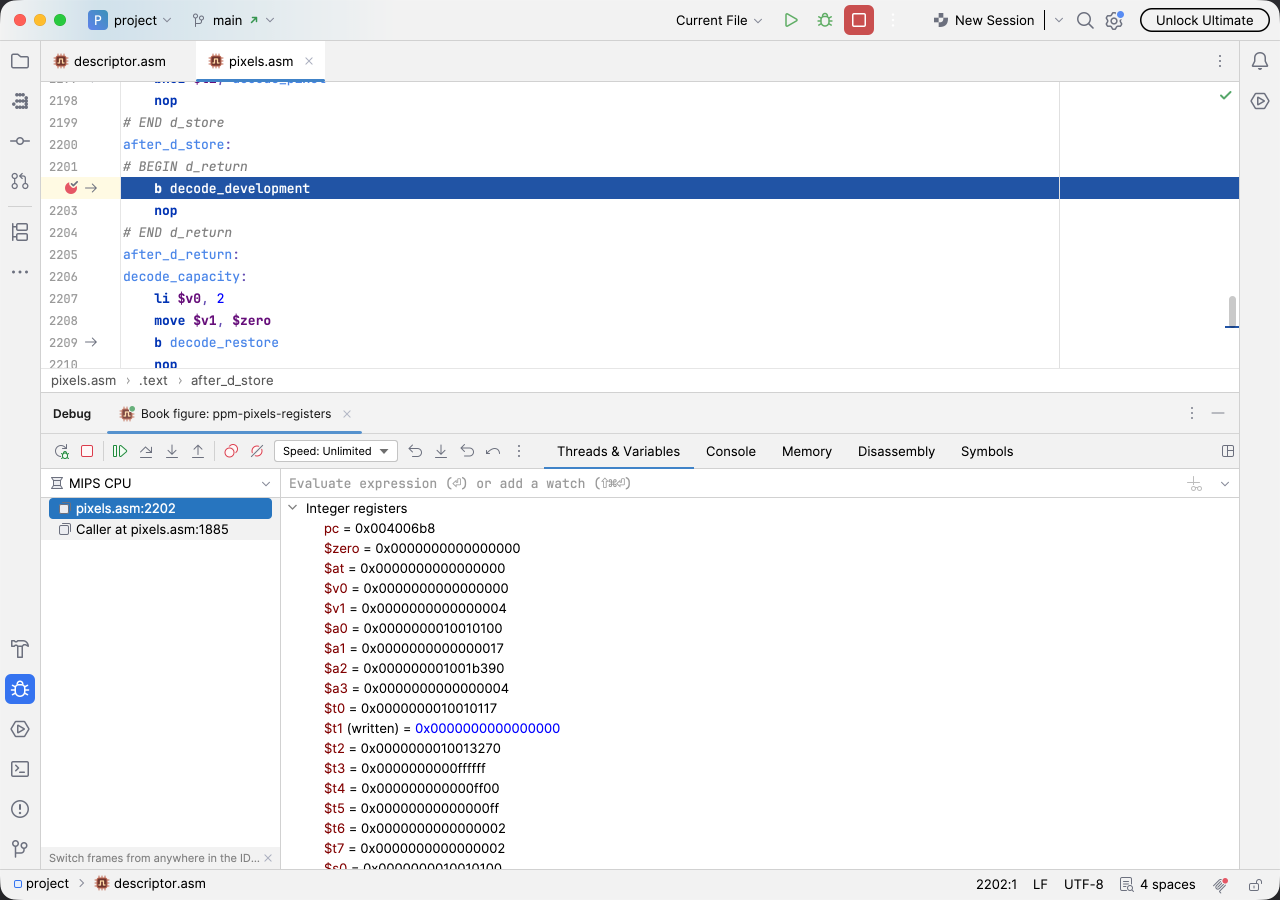
\includegraphics[width=0.6\linewidth,artifact,trim={\MARSppmpixelscursorsLeft{} \MARSppmpixelscursorsBottom{} \MARSppmpixelscursorsRight{} \MARSppmpixelscursorsTop{}},clip]{packages/029-binary-ppm/captures/f02/registers.png}};
\begin{scope}[shift={(cursors.south west)},x={($(cursors.south east)-(cursors.south west)$)},y={($(cursors.north west)-(cursors.south west)$)}]
\draw[black,line width=0.7pt] (0.023437500,0.015873016) rectangle (0.964843750,0.968253968);
\node[draw=black,fill=white,circle,inner sep=1.5pt,font=\footnotesize] at ($(0.023437500,0.968253968)+(-3mm,0)$) {2};
\end{scope}
\node[anchor=north west,inner sep=0,font=\small\bfseries] (input-title) at ([yshift=-1mm]cursors.south west) {Three bytes per source pixel};
\node[anchor=north west,inner sep=0] (input) at ([yshift=-1mm]input-title.south west) {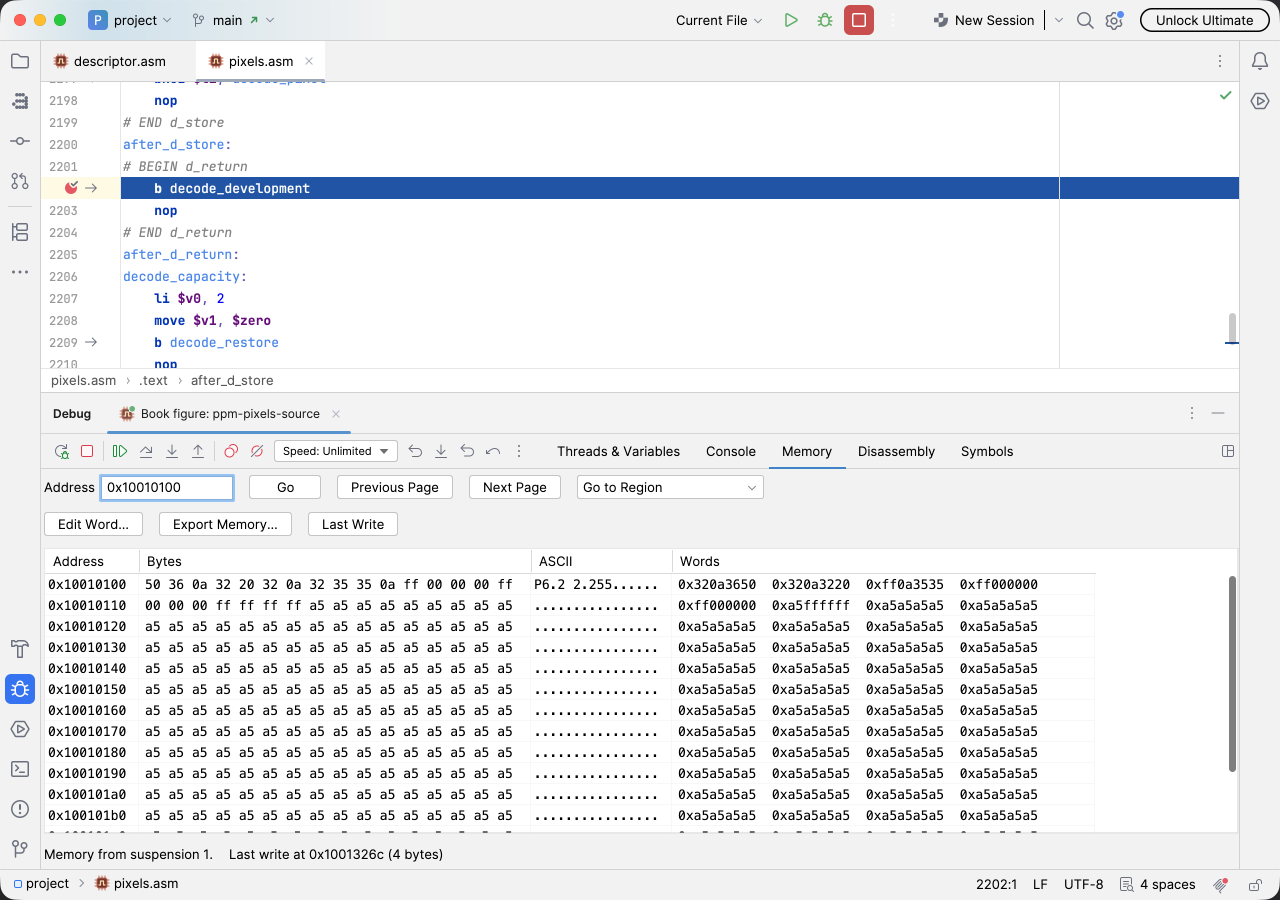
\includegraphics[width=0.84\linewidth,artifact,trim={\MARSppmpixelsinputLeft{} \MARSppmpixelsinputBottom{} \MARSppmpixelsinputRight{} \MARSppmpixelsinputTop{}},clip]{packages/029-binary-ppm/captures/f02/source.png}};
\begin{scope}[shift={(input.south west)},x={($(input.south east)-(input.south west)$)},y={($(input.north west)-(input.south west)$)}]
\draw[black,line width=0.7pt] (0.194672131,0.055555556) rectangle (0.997950820,0.638888889);
\node[draw=black,fill=white,circle,inner sep=1.5pt,font=\footnotesize] at ($(0,0.638888889)+(-3mm,0)$) {3};
\end{scope}
\node[anchor=north west,inner sep=0,font=\small\bfseries] (output-title) at ([yshift=-1mm]input.south west) {Four bytes per framebuffer pixel};
\node[anchor=north west,inner sep=0] (output) at ([yshift=-1mm]output-title.south west) {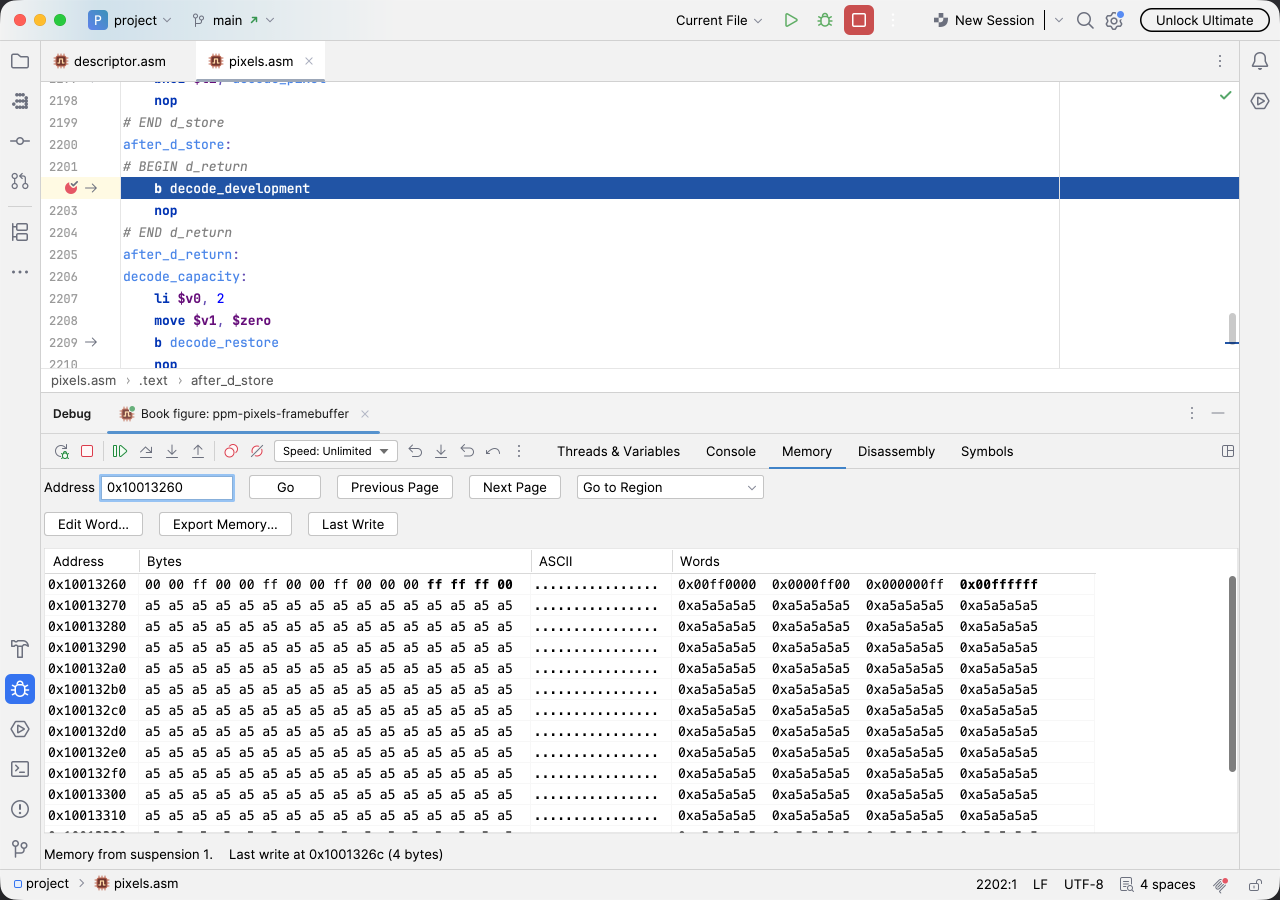
\includegraphics[width=0.84\linewidth,artifact,trim={\MARSppmpixelsoutputLeft{} \MARSppmpixelsoutputBottom{} \MARSppmpixelsoutputRight{} \MARSppmpixelsoutputTop{}},clip]{packages/029-binary-ppm/captures/f02/framebuffer.png}};
\begin{scope}[shift={(output.south west)},x={($(output.south east)-(output.south west)$)},y={($(output.north west)-(output.south west)$)}]
\draw[black,line width=0.7pt] (0.194672131,0.055555556) rectangle (0.997950820,0.638888889);
\node[draw=black,fill=white,circle,inner sep=1.5pt,font=\footnotesize] at ($(0,0.638888889)+(-3mm,0)$) {4};
\end{scope}
\node[anchor=north west,inner sep=0,font=\small\bfseries] (metadata-title) at ([yshift=-1mm]output.south west) {Validated metadata in the active frame};
\node[anchor=north west,inner sep=0] (metadata) at ([yshift=-1mm]metadata-title.south west) {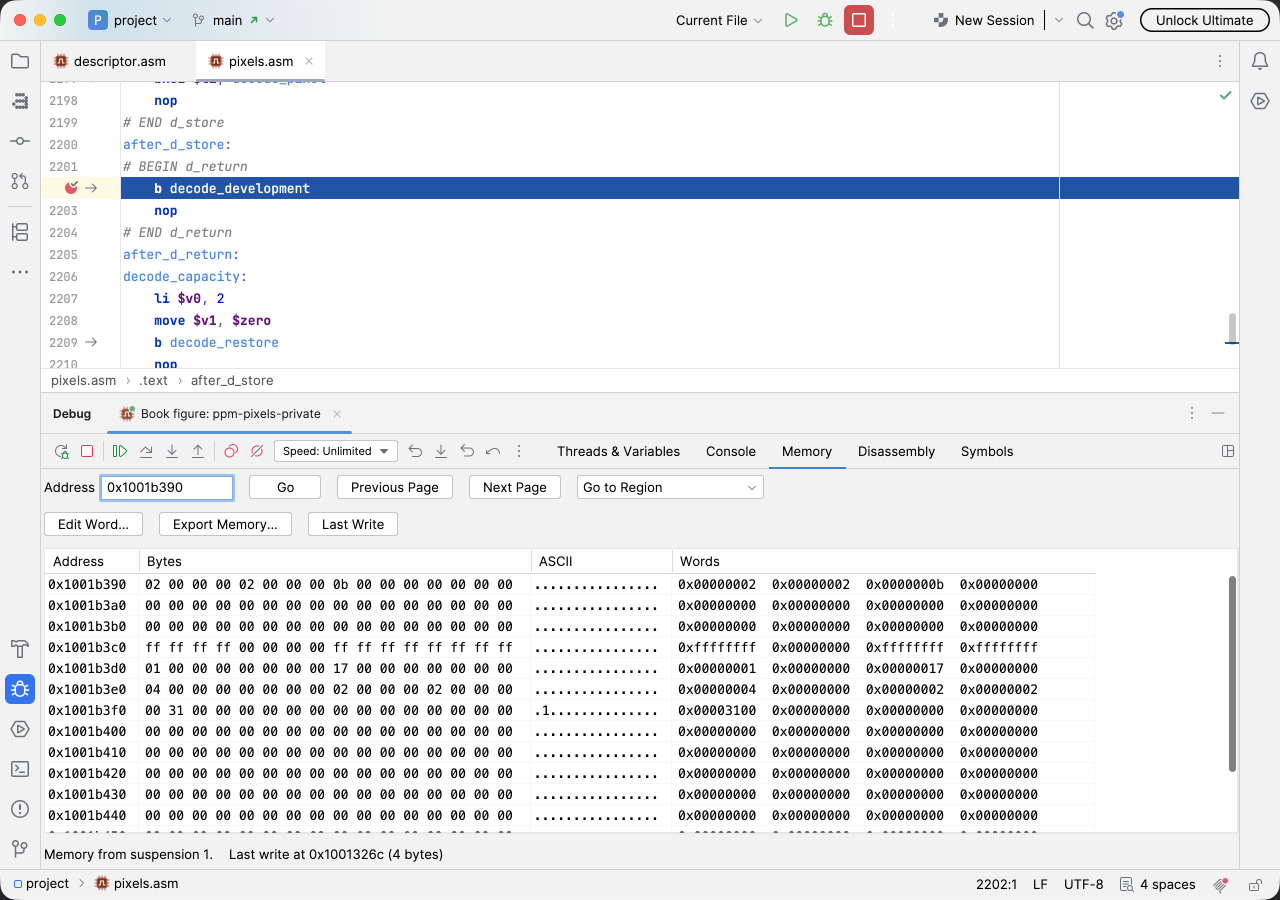
\includegraphics[width=0.84\linewidth,artifact,trim={\MARSppmpixelsmetadataLeft{} \MARSppmpixelsmetadataBottom{} \MARSppmpixelsmetadataRight{} \MARSppmpixelsmetadataTop{}},clip]{packages/029-binary-ppm/captures/f02/private.png}};
\begin{scope}[shift={(metadata.south west)},x={($(metadata.south east)-(metadata.south west)$)},y={($(metadata.north west)-(metadata.south west)$)}]
\draw[black,line width=0.7pt] (0.194672131,0.078431373) rectangle (0.997950820,0.490196078);
\node[draw=black,fill=white,circle,inner sep=1.5pt,font=\footnotesize] at ($(0,0.490196078)+(-3mm,0)$) {5};
\end{scope}
\end{tikzpicture}
\par\smallskip
\begin{minipage}{\linewidth}
\small
\begin{enumerate}
\setlength{\itemsep}{0pt}
\setlength{\parsep}{0pt}
\item This is the cumulative program through the pixel-store step. At \texttt{after\_d\_store}, the loop has finished. The next region, \texttt{d\_return}, is still the supplied development branch; successful pixel stores alone do not constitute a completed interface.
\item \texttt{t0} has reached \texttt{0x10010117}, just past the twenty-three-byte source. \texttt{t1 = 0} means that no pixels remain. \texttt{t2} has reached \texttt{0x10013270}, sixteen bytes past the framebuffer base. Each iteration advances the input by three bytes and the output by four.
\item The raster starts eleven bytes into the source. Its RGB triples describe red, green, blue and white. Bytes after the twenty-three-byte logical file remain \texttt{a5}; the decoder must not treat them as another pixel.
\item The first sixteen framebuffer bytes encode \texttt{0x00ff0000}, \texttt{0x0000ff00}, \texttt{0x000000ff} and \texttt{0x00ffffff}. Little-endian memory places each word\textquotesingle s least significant byte first. The next row remains \texttt{a5}, outside the four-pixel output.
\item The private descriptor contains width two, height two and offset eleven. It belongs to the active stack frame, not to the caller\textquotesingle s metadata arena. Continuing restores the saved registers and returns development status four with count zero. The next lesson replaces that return stub.
\end{enumerate}
\end{minipage}
\caption{The decoder has stored four pixels before its final return is implemented.}
\label{capture:029-binary-ppm-f02}
\label{ppm-f02}
\end{figure}
\par
